\documentclass[a4paper]{article}
\usepackage[T1]{fontenc}			% pacchetto per \chapter
\usepackage[italian]{babel}
\usepackage[italian]{isodate}  		% formato delle date in italiano
\usepackage{graphicx}				% gestione delle immagini
\usepackage{amsfonts}
\usepackage{booktabs}				% tabelle di qualità superiore
\usepackage{amsmath}				% pacchetto matematica
\usepackage{enumitem}				% gestione delle liste
\usepackage{pifont}					% pacchetto con elenchi carini
\usepackage{listings}				% pacchetto per i codici
\usepackage[x11names]{xcolor}		% pacchetto colori RGB
% Link ipertestuali per l'indice
\usepackage{xcolor}
\usepackage[linkcolor=black, citecolor=blue, urlcolor=cyan]{hyperref}
\hypersetup{
	colorlinks=true
}

\newcommand{\longline}{\noindent\rule{\textwidth}{0.4pt}}
\newcommand{\dquotes}[1]{``#1''}

\definecolor{codegreen}{rgb}{0,0.6,0}
\definecolor{codegray}{rgb}{0.5,0.5,0.5}
\definecolor{codepurple}{rgb}{0.58,0,0.82}
\definecolor{backcolour}{rgb}{0.95,0.95,0.92}
\lstdefinestyle{mystyle}{
	backgroundcolor=\color{backcolour},   
	commentstyle=\color{codegreen},
	keywordstyle=\color{magenta},
	numberstyle=\tiny\color{codegray},
	stringstyle=\color{codepurple},
	basicstyle=\ttfamily\footnotesize,
	breakatwhitespace=false,         
	breaklines=true,                 
	captionpos=b,                    
	keepspaces=true,                 
	numbers=left,                    
	numbersep=5pt,                  
	showspaces=false,                
	showstringspaces=false,
	showtabs=false,                  
	tabsize=2
}

\lstdefinelanguage{JavaScript}{
	keywords={typeof, new, true, false, catch, function, return, null, catch, switch, var, if, in, while, do, else, case, break},
	keywordstyle=\color{blue}\bfseries,
	ndkeywords={class, export, boolean, throw, implements, import, this},
	ndkeywordstyle=\color{darkgray}\bfseries,
	identifierstyle=\color{black},
	sensitive=false,
	comment=[l]{//},
	morecomment=[s]{/*}{*/},
	commentstyle=\color{codegreen}\ttfamily,
	stringstyle=\color{red}\ttfamily,
	morestring=[b]',
	morestring=[b]"
}

\lstset{
	language=JavaScript,
	backgroundcolor=\color{lightgray},
	extendedchars=true,
	basicstyle=\footnotesize\ttfamily,
	showstringspaces=false,
	showspaces=false,
	numbers=left,
	numberstyle=\footnotesize,
	numbersep=9pt,
	tabsize=2,
	breaklines=true,
	showtabs=false,
	captionpos=b
}

\lstset{style=mystyle}

%\usepackage{showframe}				% visualizzazione bordi
%\usepackage{showkeys}				% visualizzazione etichetta

\begin{document}
	\author{VR443470 - Valentini Andrea}
	\title{Università degli studi di Verona \\
		\:\\
		Tesina su FaaS (Function-as-a-Service)}
	\date{\printdayoff\today}
	\maketitle
	
	\newpage
	
	% indice
	\tableofcontents
	
	\newpage
	
	\section{Introduzione}
	
	Con l'avanzare della tecnologia e del \emph{cloud computing}, è aumentata sempre di più la richiesta di servizi online che consentissero di utilizzare calcolatori già pronti e con grandi disponibilità di calcolo.
	
	La crescita del \emph{cloud computing} è stata esponenziale nell'ultimo decennio, soprattutto anche grazie, purtroppo, alla pandemia del COVID-19. Tant'è che il CEO di Microsoft, Satya Nadella, disse:
	\begin{center}
		\dquotes{\emph{We’ve seen two years of digital transformation in two months.}}
	\end{center}
	
	\longline
	
	% https://www.ibm.com/topics/faas#What+is+FaaS%3F
	% https://www.redhat.com/en/topics/cloud-native-apps/what-is-faas#overview
	\subsection{Che cos'è FaaS}
	
	Function-as-a-Service (FaaS) è una tipologia (\emph{event-driven}) di servizio \emph{cloud computing} che consente ai programmatori di sviluppare, eseguire e gestire pacchetti di applicazioni come se fossero funzioni, senza preoccuparsi della manutenzione di una propria infrastruttura.
	
	Tipicamente, l'\emph{hosting} di un'applicazione software su Internet richiede: la gestione di un server virtuale o fisico e la gestione di un sistema operativo. Con FaaS, viene tutto gestito in automatico dal \emph{cloud service provider}.
	
	\begin{figure}[!htp]
		\centering
		
\includegraphics[width=\textwidth]{img/faas-1.jpg}
	\end{figure}
	
	\noindent
	I vantaggi di questa tecnologia sono molteplici e verranno spiegati più avanti. Per esempio, i programmatori possono concentrarsi solamente sul codice delle loro applicazioni.
	
	\newpage
	
	% https://www.ibm.com/topics/faas#FaaS+vs.+serverless
	% https://www.redhat.com/en/topics/cloud-native-apps/what-is-faas#faas-and-serverless
	\subsection{FaaS e serverless}
	
	\emph{Serverless} è un modello di sviluppo ed esecuzione di applicazioni di \emph{cloud computing}, il quale consente ai programmatori di costruire ed eseguire il codice dell'applicazione senza preoccuparsi dei server o del \emph{backend} dell'infrastruttura.
	
	Nonostante spesso le persone scambino i modelli serverless e FaaS tra di loro, la verità è che sono due concetti diversi ed è più corretto dire che FaaS è un sottoinsieme dei modelli serverless.
	\begin{figure}[!htp]
		\centering
		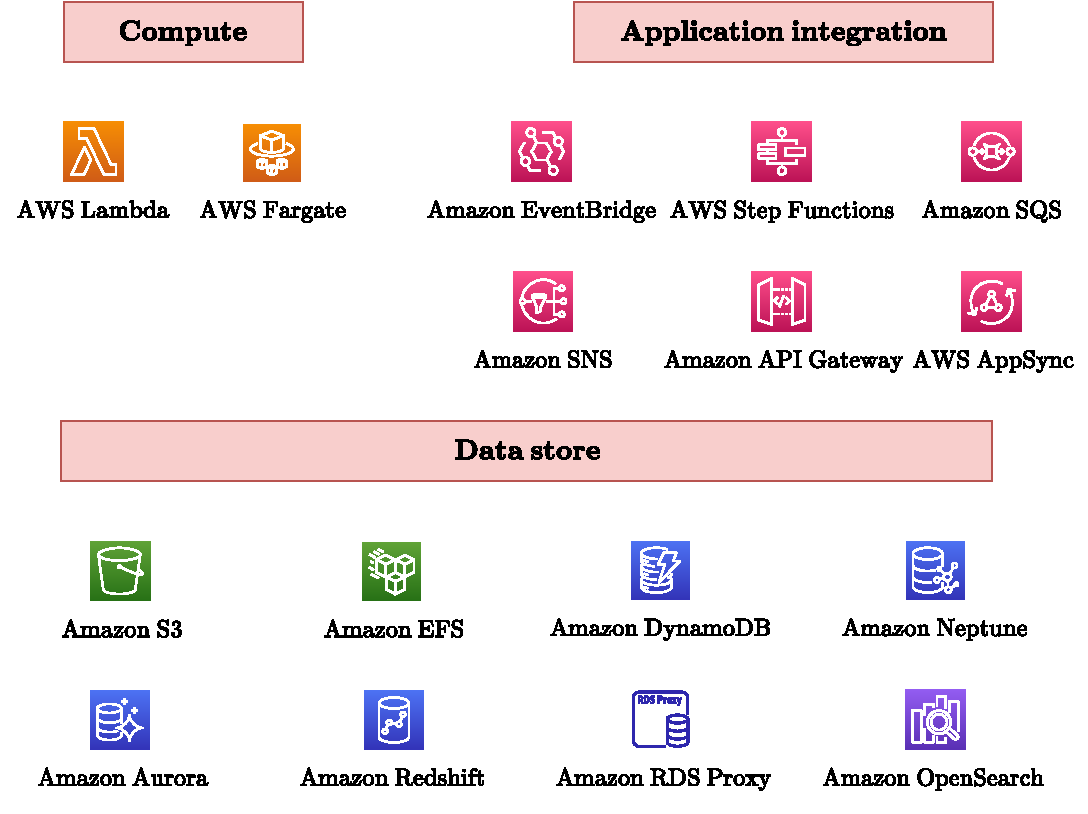
\includegraphics[width=\textwidth]{img/AWS-Serverless-1.pdf}
		\caption{Esempio dei vari servizi \emph{serverless} offerti da Amazon.}
		\label{fig: AWS serverless services}
	\end{figure}
	
	\noindent
	Il modello \emph{serverless} è focalizzato su \textbf{qualsiasi} categoria di servizio, come la computazione, l'archiviazione, i database, la messaggistica, le \emph{api gateways}\footnote{Un \emph{api gateway} è uno strumento di gestione delle API che si trova tra un client e una raccolta di servizi back-end.}, etc. In tutti queste categorie, la configurazione, la gestione e il costo effettivo dei server, è nascosto all'utente finale.
	
	La figura~\ref{fig: AWS serverless services} dovrebbe dimostrare come il servizio FaaS sia solo un sottoinsieme dell'enorme modello \emph{serverless}. Amazon, come verrà anche approfondito più avanti, come servizio FaaS propone AWS Lambda.\newline
	
	Il modello Function-as-a-Service può essere considerato la tecnologia più centrale nell'architettura \emph{serverless}. In altre parole è il cuore pulsante. FaaS è focalizzato sul paradigma \emph{event-driven} (orientato agli eventi), dove il codice dell'applicazione, o del \emph{container}, viene eseguito solo in risposta a determinati eventi o richieste.\newpage
	
	\section{Aziende che offrono un servizio FaaS}
	
	\subsection{IBM: cloud functions}
	
	\subsubsection{Panoramica}
	
	L'azienda IBM offre come servizio FaaS \href{https://cloud.ibm.com/functions/}{IBM Cloud Functions} e si basa su Apache OpenWhisk\footnote{Apache OpenWhisk è una piattaforma open source che consente di eseguire funzioni in risposta ad eventi.}. 	
	
	Cloud Functions è diverso dalle tecnologie di calcolo tradizionali; si paga solo per il tempo per cui il codice sta soddisfacendo le richieste, arrotondato al 100ms più vicino. Questo significa che si potrebbero vedere dei notevoli risparmi rispetto ad altre tecnologie come le macchine virtuali e i contenitori, che probabilmente non sono utilizzati al 100\% pur continuando a utilizzare memoria sul sistema del provider cloud.
	
	Cloud Functions viene fatturato al secondo per gigabyte di memoria. Questo significa che è possibile ulteriormente ridurre i costi allocando solo la quantità di memoria necessaria perché le funzioni svolgano il loro lavoro.
	\begin{figure}[!htp]
		\centering
		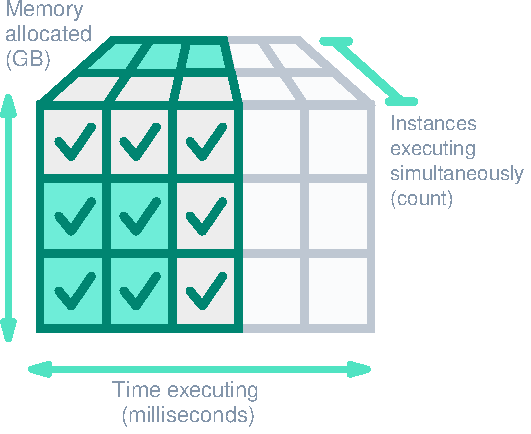
\includegraphics[width=.6\textwidth]{img/IBM-1.pdf}
		\caption{Funzionamento del calcolo del costo di IBM Cloud Functions.}
	\end{figure}
	
	\begin{table}[!htp]
		\centering
		\begin{tabular}{@{} l l l l @{}}
			\toprule
			Tempo esec. azione & Memoria dell'azione & Esecuzioni al mese & Costo al mese \\
			\midrule
			500ms	& 128MB & 5.000.000		& Gratuito \\
			500ms	& 256MB & 5.000.000		& \$4,00 \\
			500ms	& 512MB & 5.000.000		& \$15,10 \\
			1.000ms	& 128MB & 10.000.000	& \$15,10 \\
			1.000ms	& 256MB & 10.000.000	& \$37,31 \\
			1.000ms	& 512MB & 10.000.000	& \$81,72 \\
			\bottomrule
		\end{tabular}
		\caption{Stima di costi a seconda dell'utilizzo}
	\end{table}
	
	\subsubsection{Caso studio: GreenQ}
	
	Tra tutti i casi studio che propone l'azienda IBM sul proprio sito, ne esistono 3 che riguardano singolarmente la tecnologia FaaS: GreenQ, Articoolo e SiteSpirit. Si approfondisce l'azienda GreenQ.\newline
	
	\noindent
	La GreenQ Ltd. è un'azienda americana (Santa Monica, California) che ha l'obbiettivo di portare la tecnologia IoT (Internet of Things) al servizio dei municipi in cui gestiscono i rifiuti delle città americane.
	
	\begin{figure}[!htp]
		\centering
		
\includegraphics[width=.5\textwidth]{img/GreenQ-logo.pdf}
	\end{figure}
	
	\noindent
	\textbf{\emph{La sfida da superare.}} I municipi spendono cifre significative per raccogliere i rifiuti, ma spesso potrebbero essere ammortizzati eseguendo un'ottimizzazione dei processi.
	
	L'azienda GreenQ sfrutta tale gap per introdurre una piattaforma IoT che consenta di salvare dati, come il tempo di ritiro, la posizione e il peso del cestino, grazie a schede hardware sui furgoni dell'immondizia. Questi dispositivi inviavano i dati all'azienda GreenQ per monitorarli e analizzarli così da migliorare l'organizzazione delle gestione del ritiro dei rifiuti. Tuttavia, dopo il lancio di un prototipe, l'azienda ha iniziato a ripensare alla sua architettura e infrastruttura.
	
	Edy Candel, il CTO (\emph{Chief Technology Officier}) e cofondatore di GreenQ, disse: \dquotes{\emph{Dopo aver assunto i primi clienti, ci rendemmo conto che stavamo spendendo tanto tempo nel gestire le nostre virtual machines e aggiungere potenza computazionale. Vedemmo che la nostra infrastruttura aveva un numero di richieste che dipendevano dal numero di clienti e camion che stavano lavorando, quindi ci rendemmo conto che era difficile ottenere la scalabilità desiderata}}.\newline
	
	\noindent
	\textbf{\emph{La trasformazione.}} GreenQ entra a far parte del programma \dquotes{IBM Alpha Zone Accelerator} creato appositamente per le \emph{startup}. Così facendo, viene eseguita una migrazione dalla vecchia architettura alla FaaS di IBM, ovvero la IBM Cloud Functions.
	
	Dato il paradigma event-driven, ad ogni pezzo dell'applicazione di GreenQ viene assegnato un trigger a seconda dell'azione scatenata o dell'insieme di azioni scatenate, eliminando in questo modo l'attivazione manuale nel \emph{workflow}. Per esempio, quando il sensore del furgone dell'immondizia raccoglie dati da un cestino dei rifiuti durante il prelievo, l'evento \emph{triggera} la soluzione adottata da GreenQ per controllare, analizzare e salvare automaticamente le informazioni.
	
	Ultimamente, la piattaforma \emph{cloud-based} fornita ai municipi e ad altre organizzazioni di raccolta dei rifiuti, è stata migliorata inserendo una \emph{dashboard} in cui è possibile visualizzare in tempo reale: la posizione e il percorso dei furgoni della spazzatura, inviare e ricevere notifiche, e analizzare i dati per migliorare i servizi. Per continuare ad evolvere la sua offerta, GreenQ prevede di incorporare altre tecnologie di IBM, come IBM Watson Visual Recognition, per catturare e tradurre informazioni visive sui percorsi di ritiro dei clienti.
	
	\subsection{Amazon: AWS Lambda}
	
	\subsubsection{Panoramica}
	
	L'azienda Amazon offre come servizio FaaS \href{https://aws.amazon.com/lambda/?nc2=h_ql_prod_fs_lbd}{AWS Lambda}. Inoltre, Amazon offre più di 200 servizi AWS e \emph{Software-as-a-Service} (SaaS) che consentono di \emph{triggerare} AWS Lambda.
	\begin{figure}[!htp]
		\centering
		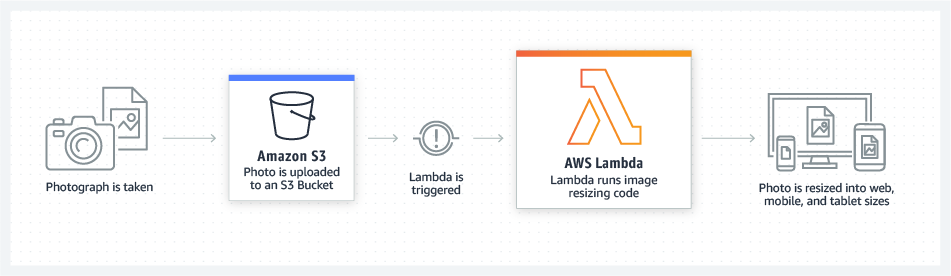
\includegraphics[width=\textwidth]{img/AWS-Lambda-1.png}
		\caption{Esempio di utilizzo di AWS Lambda. Utilizzando il servizio di Data Store chiamato Amazon S3 è possibile salvare una foto carica da un utente, \emph{triggerare} AWS Lambda e quest'ultimo eseguire l'azione di ridimensionamento dell'immagine.}
	\end{figure}
	
	\noindent
	Su AWS Lambda è possibile scegliere se eseguire le funzioni su processori x86 o architetture Arm. Il prezzo varia a seconda delle architetture e quindi si rimanda al sito ufficiale: \url{https://aws.amazon.com/it/lambda/pricing/}
	
	\longline
	
	\subsubsection{Caso studio: Coca-Cola}
	
	Tra la marea di casi studio proposti dall'azienda Amazon, qua di seguito viene proposto quello di Coca-Cola Company.\newline
	
	\noindent
	La Coca-Cola Company è un'azienda statunitense (Atlanta, Georgia) ed è una delle più grandi aziende produttrici e distributrici di bevande analcoliche e concentrati di sciroppi a livello mondiale.
	\begin{figure}[!htp]
		\centering
		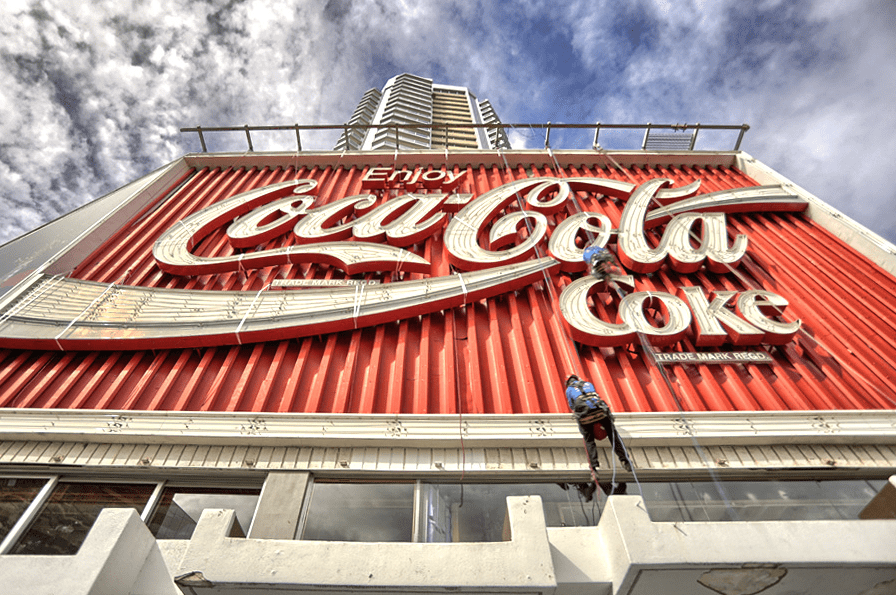
\includegraphics[width=.4\textwidth]{img/Coca-Cola-1.png}
	\end{figure}\newpage
	
	\noindent
	\textbf{\emph{La sfida da superare.}} Nel 2020, il mondo è stato colpito da una pandemia chiamata COVID-19. Questa tragedia ha provocato un grosso cambiamento nel comportamento degli esseri umani e l'azienda Coca-Cola stava cercando di migliorare i suoi distributori chiamati \dquotes{Coca-Cola Freestyle}.
	\begin{figure}[!htp]
		\centering
		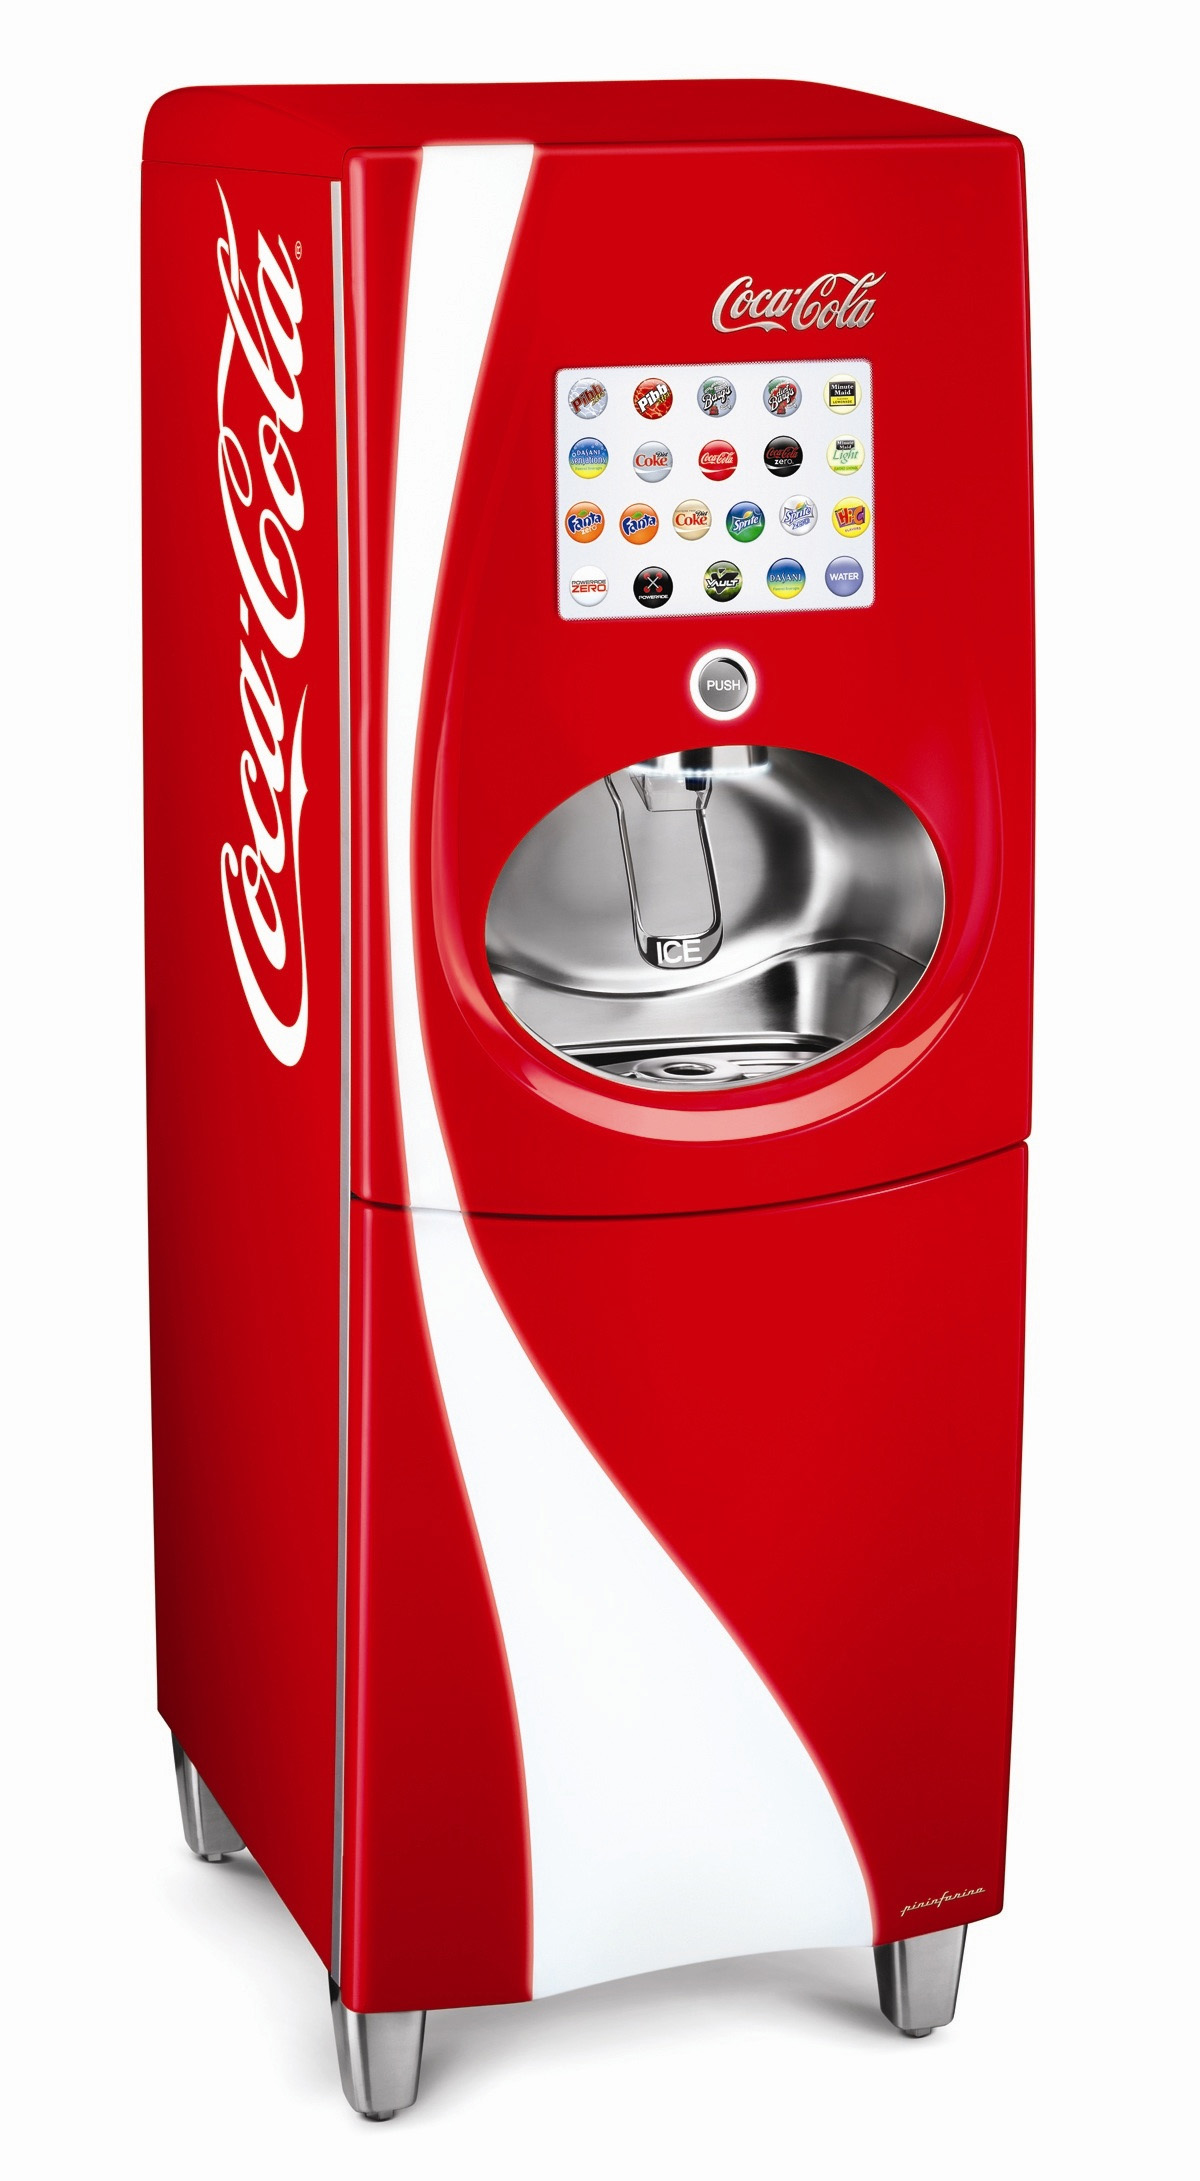
\includegraphics[width=.3\textwidth]{img/Coca-Cola-2.jpg}
		\caption{Coca-Cola Freestyle.}
	\end{figure}
	
	\noindent
	Thomas Stubbs, vie presidente dell'ingegneria e dell'innovazione al \emph{Coca-Cola Freestyle Equipment Innovation Center}, ha affermato: \dquotes{\emph{Tutti i dispenser Coca-Cola sono sicuri grazie ad una minuziosa cura e pulizia. Ma in questi periodi incerti, Coca-Cola vuole proporre ai clienti una nuova opzione: un'esperienza touchless}}. Per \emph{touchless} si intende un distributore che non necessita di essere toccato, quindi limitando al massimo il contatto tra le persone.\newline
	
	\noindent
	\textbf{\emph{La realizzazione.}} Per realizzare l'idea di Coca-Cola, la bassa latenza (\emph{low latency}) era la chiave essenziale. Per questo motivo, Amazon ha pensato di adottare la sua AWS \emph{serverless architecture} al nuovo distributore \emph{contactless} così da far scegliere la bibita desiderata ai clienti tramite il proprio \emph{smartphone} in pochi secondi \textbf{senza} il bisogno di scaricare un'applicazione o avere un account!
	
	Il team Freestyle ha creato una web app \emph{serverless} che si integrava con i distributori Coca-Cola Freestyle, in appena 4 mesi.\newpage
	
	\subsection{Google: cloud functions}
	
	\subsubsection{Panoramica}
	
	L'azienda Google offre come servizio FaaS \href{https://cloud.google.com/functions/}{Google Cloud Functions}. Nel complesso sembra un servizio come gli altri, ma il sito fornisce una grande documentazione facilmente consultabile e una serie di casi d'uso.
	\begin{figure}[!htp]
		\centering
		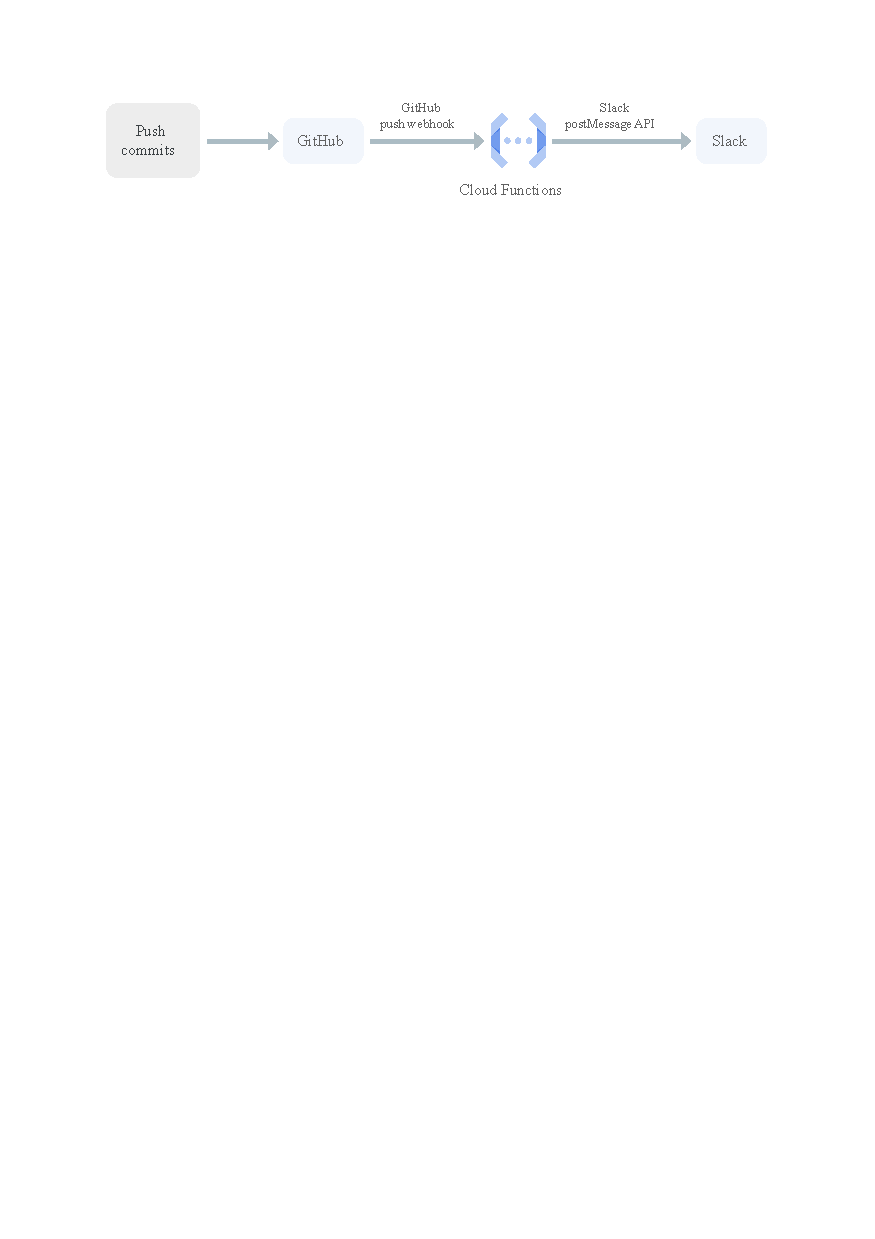
\includegraphics[width=\textwidth]{img/Google-1.pdf}
		\caption{Esempio di caso d'uso: integrazione con servizi di terze parti e APIs.}
	\end{figure}
	
	\noindent
	Il prezzo varia a seconda dell'utilizzo che se ne fa: \url{https://cloud.google.com/functions/pricing}
	
	\longline
	
	\subsubsection{Caso studio: Commerzbank}
	
	Tra i vari casi studio proposti da Google, qua di seguito viene approfondito Commerzbank.\newline
	
	\noindent
	La Commerzbank è la quarta più grande banca della Germania, dopo Deutsche Bank, DZ Bank e KfW, con sede a Francoforte sul Meno, fondata nel 1870 ad Amburgo.
	\begin{figure}[!htp]
		\centering
		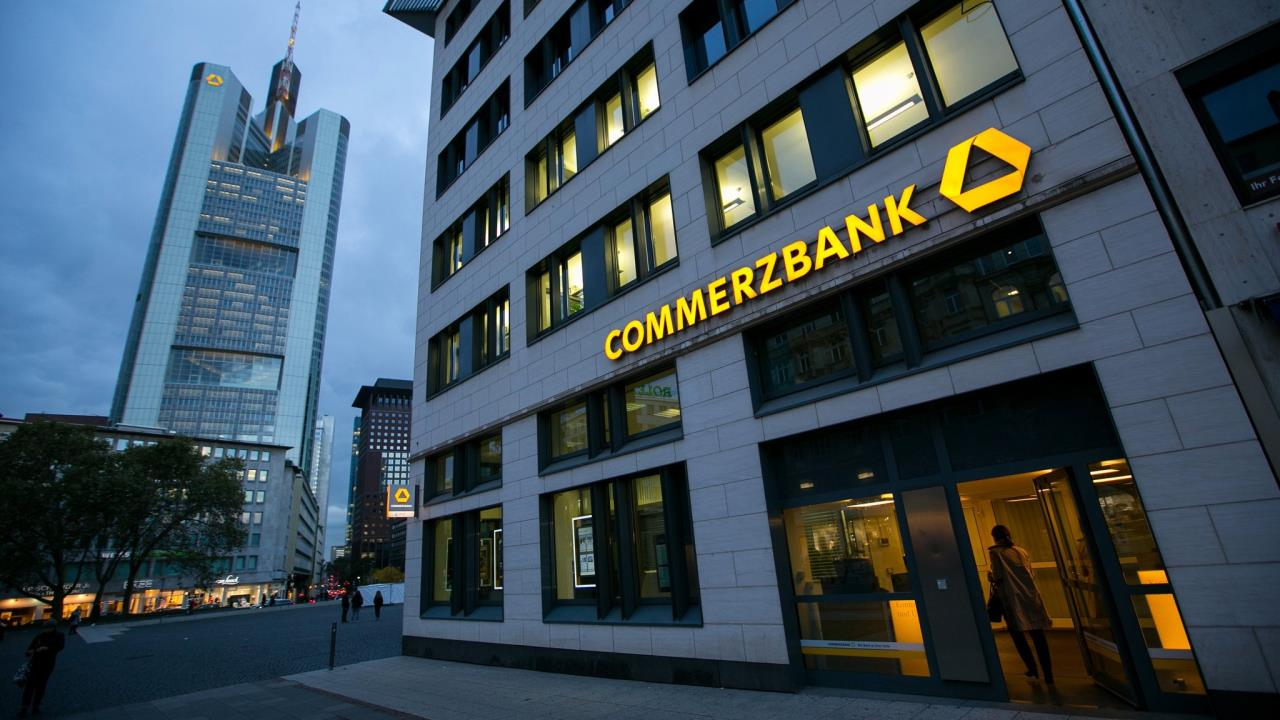
\includegraphics[width=\textwidth]{img/Googe-2.jpg}
		\caption{Foto della sede tedesca Commerzbank.}
	\end{figure}\newpage
	
	\noindent
	\textbf{\emph{La sfida da superare.}} L'83\% dei servizi finanziari, secondo Google Cloud survey, vengono sviluppati utilizzando servizi cloud. Per alcune banche, tra cui Commerzbank, la sicurezza è un aspetto fondamentale e questo cambiamento ha influito su tale aspetto. Le aziende che forniscono servizi finanziari devono maneggiare una grande quantità di dati sensibili che non possono essere compromessi.
	
	Gli standard di sicurezza che sono cresciuti negli ultimi dieci anni, non possono essere spostati in massa all'interno del cloud, ma devono essere ridisegnati.
	\begin{center}
		\dquotes{\emph{Un fattore critico della nostra adozione della tecnologia cloud, è sempre stato le varie funzionalità che il cloud porta con sé quando deve processare una grande quantità di dati, per esempio, per ricavare informazioni dettagliate. Al momento del salvataggio in cloud, abbiamo bisogno di essere sicuri che i dati siano protetti e rispettino gli stretti standard di sicurezza. Questo è il motivo per cui abbiamo scelto Google Cloud.}}\newline
		
		\noindent
		- \emph{Christian Gorke, Head of Cyber Center of Excellence, Commerzbank}
	\end{center}\:\newline
	
	\noindent
	\textbf{\emph{La realizzazione.}} Il nuovo sistema di sicurezza implementato da Google è implementato all'interno (\emph{built-in}). Questo si traduce in un'automatizzazione in larga scala, poiché i dipendenti non dovranno preoccuparsi di configurare software complessi come firewall, ma sarà tutto automatizzato da Google. Questo approccio viene chiamato \emph{invisible security}.
	
	Gorke spiega come funziona: \dquotes{La sicurezza invisibile di Commerzbank è un approccio diviso in 4 passaggi. Primo, viene azionato Cloud Logging e Asset Inventory per ottenere una panoramica completa di tutte le nostre risorse nel cloud. Dopodiché, si implementa un filtro e uno strato d'azione basato sul modello Pub/Sub e BigQuery, i quali ci consentono di definire programmaticamente un ampio range di sicurezza per i vari casi d'uso. Successivamente, si valutano le misure corrette di sicurezza basate sugli eventi scatenati utilizzando Cloud Functions e Cloud Run, a seconda sempre dei casi d'uso. Dopo troviamo le misure di sicurezza corretti con BigQuery e Cloud Functions. Infine, eseguiamo un report dei risultati al Security Command Center.}
	
	La soluzione di automatizzazione dei livelli di sicurezza di Google, consente ai dipendenti di Commerzbank di focalizzarsi sul proprio lavoro invece che sui possibili problemi di sicurezza.\newpage
	
	\subsection{Microsoft: Azure functions}
	
	\subsubsection{Panoramica}
	
	L'azienda Microsoft offre come servizio FaaS \href{https://azure.microsoft.com/en-us}{Microsoft Azure}. Sul proprio sito, Microsoft presenta le varie potenzialità del proprio servizio. Inoltre, Microsoft afferma che il proprio servizio è 5 volte più economico del concorrente Amazon: \url{https://azure.microsoft.com/en-us/pricing/}
	\begin{figure}[!htp]
		\centering
		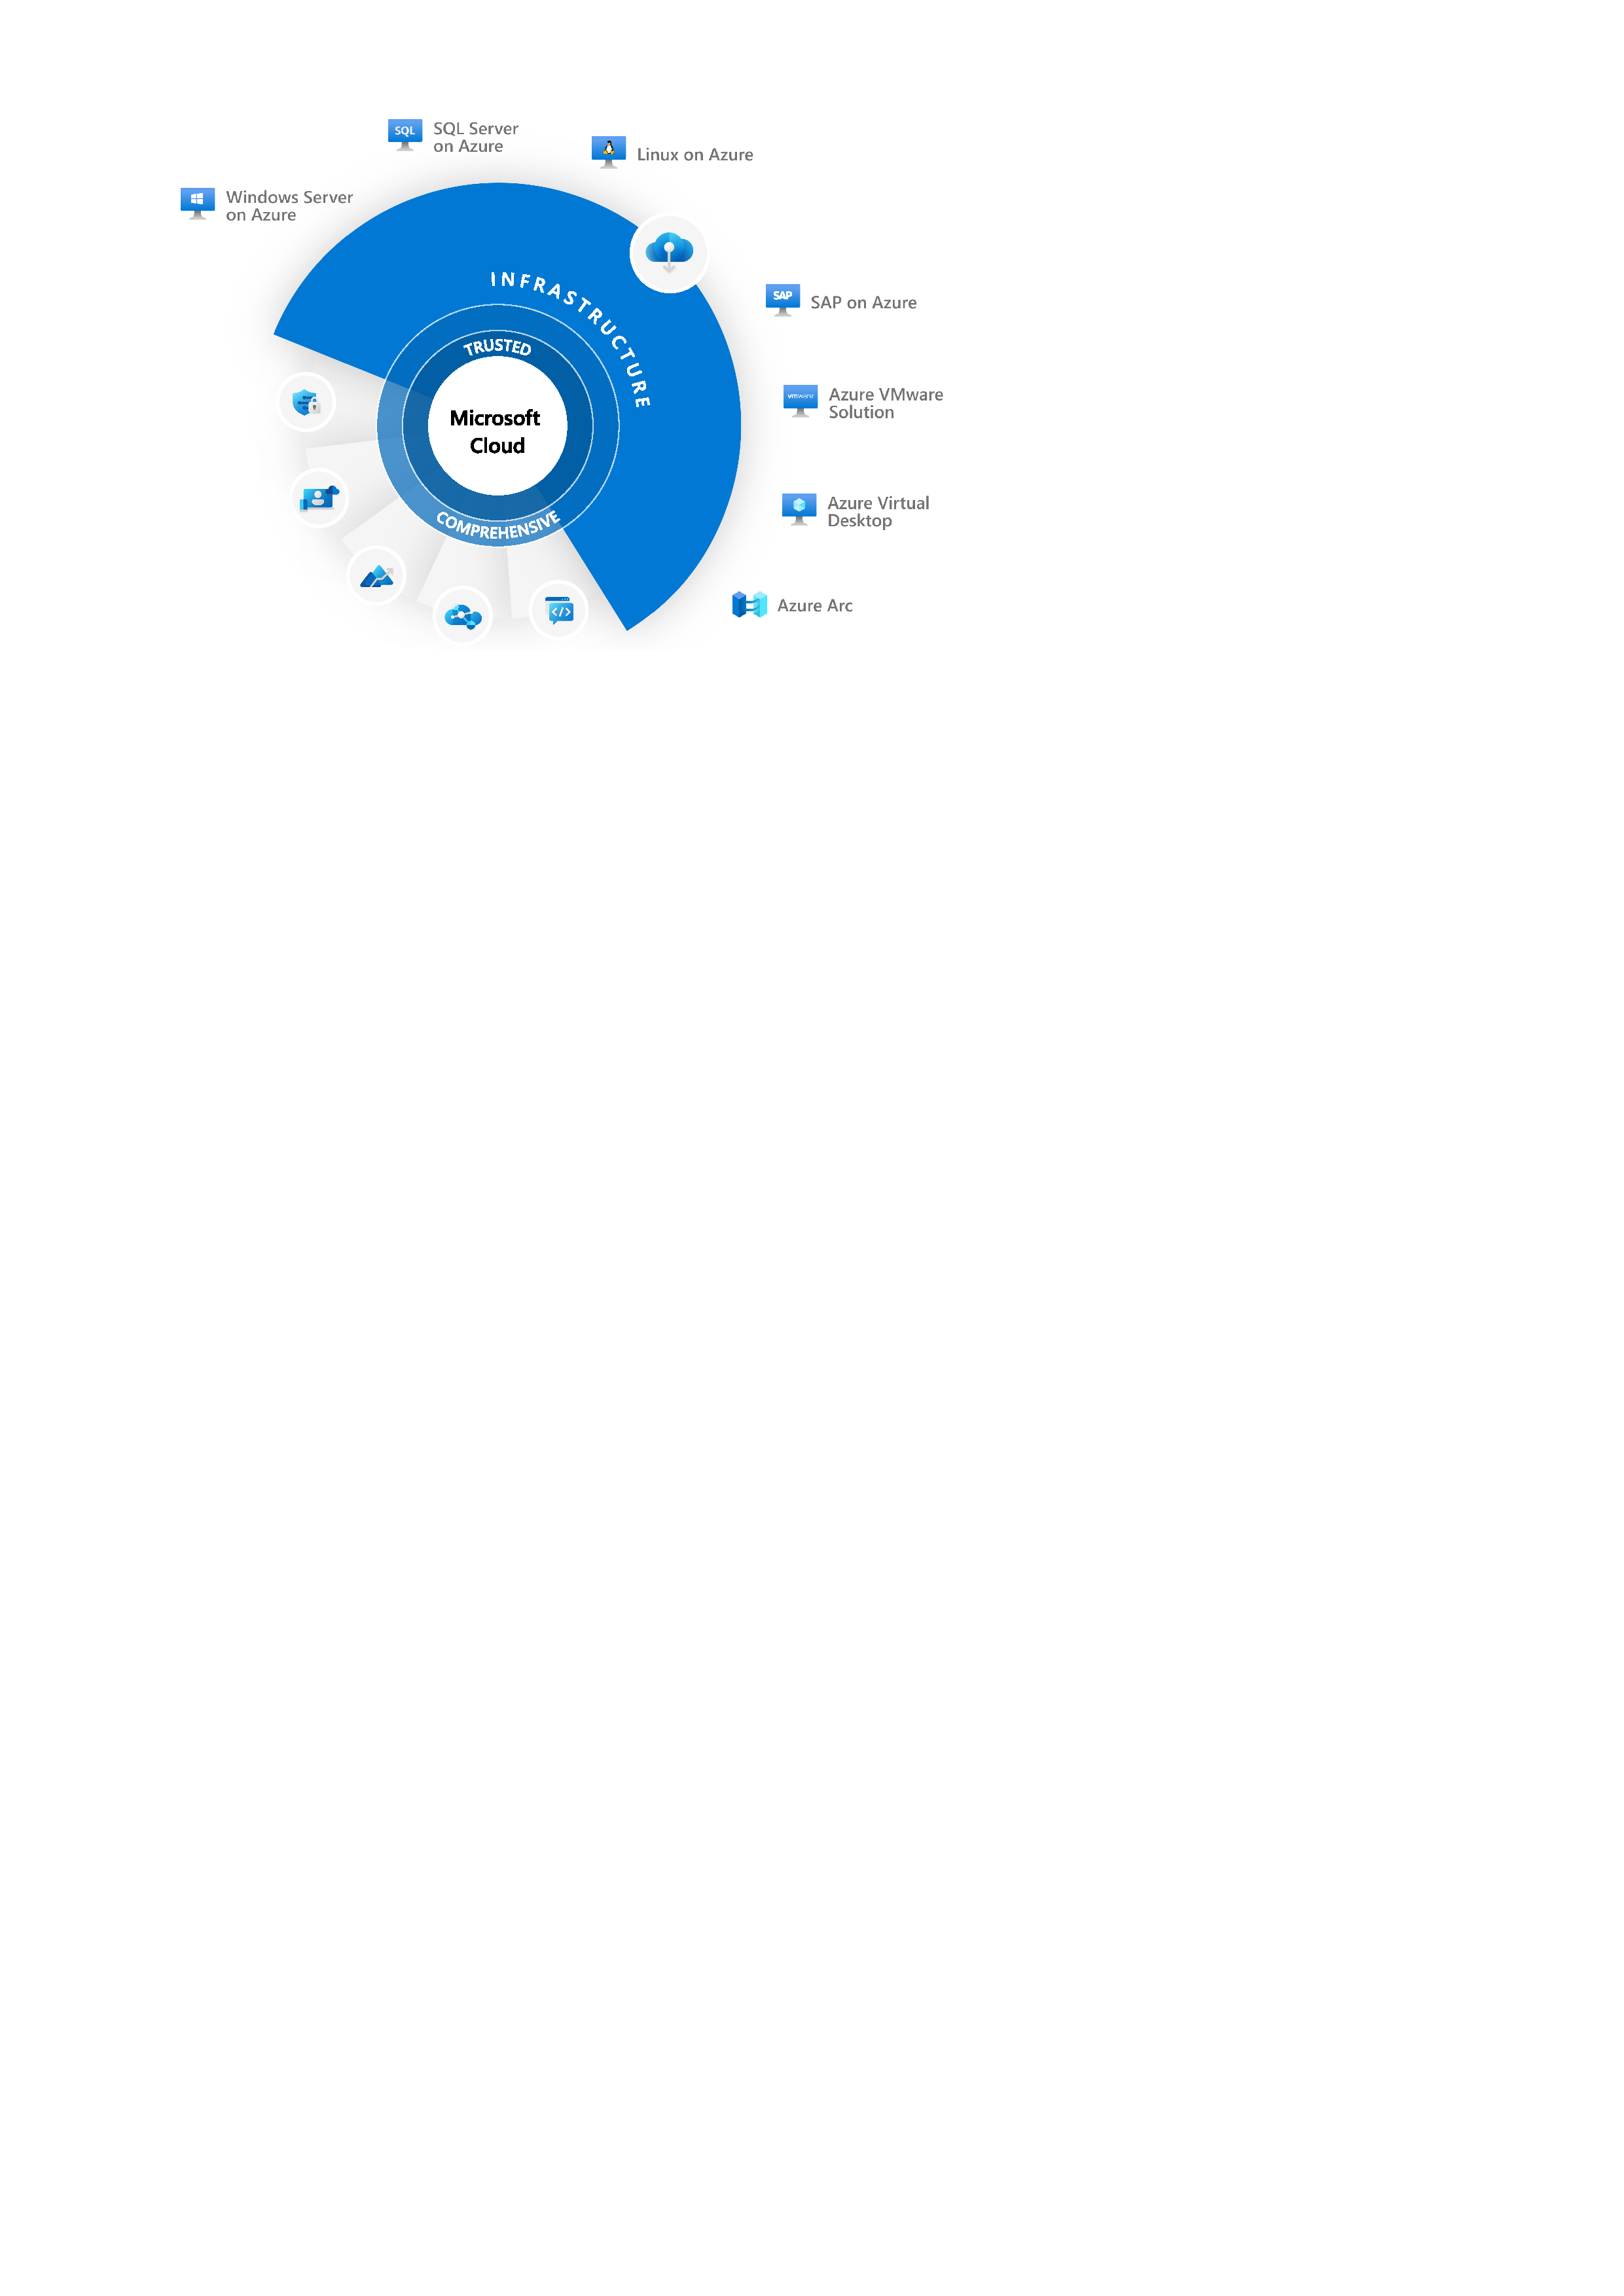
\includegraphics[width=\textwidth]{img/Microsoft-1.pdf}
		\caption{Infrastruttura di Azure.}
	\end{figure}\newpage
	
	\subsubsection{Caso studio: Fujitsu}
	
	Tra le aziende più famose con cui ha lavorato Microsoft, si presenta qua di Seguito Fujitsu.\newline
	
	\noindent
	Fujitsu è un'azienda giapponese con sede a Tokyo e Kawasaki. È uno dei maggiori fornitori mondiali di prodotti e servizi per l'\emph{information technology}, dai personal computer, midrange, grandi server e sistemi di storage, fino al software.
	\begin{figure}[!htp]
		\centering
		
\includegraphics[width=\textwidth]{img/Fujitsu-1.jpg}
		\caption{Logo di Fujitsu.}
	\end{figure}
	
	\subsection{Oracle: OCI}
	
	\subsubsection{Panoramica}
	
	\subsubsection{Caso studio}
	
	\subsubsection{Prezzo del servizio}
	
	\section{Esempio di applicazione}	
\end{document}